\documentclass[12pt]{article}
\usepackage[pdftex]{graphicx}
\begin{document}
\newcounter{problem}
\thispagestyle{empty}

\section*{NYU General Physics 1---Problem set 2}

\paragraph{Problem~\theproblem:}\refstepcounter{problem}%
What is the mean acceleration $a$ of a dragster (that is, a
drag-racing automobile) that can travel 0.25~mi in 5.5~s, starting
from a dead stop?  Assume that the dragster accelerates with constant
acceleration throughout the 5.5~s (not a terrible assumption, but not
a good one either).  Give your answer in terms of the gravitational
acceleration $g$.  Does your answer seem reasonable?  What do you
predict, under the constant-acceleration assumption, for the final
speed $v_\mathrm{f}$ of the dragster as it crosses the finish line?
Convert your answer to $\mathrm{mi\,h^{-1}}$.  Search the web for the
current world-record quarter-mile drag-race time and final speed.

\paragraph{Problem~\theproblem:}\refstepcounter{problem}%
For the time interval $0<t<1~\mathrm{s}$, draw graphs of the vertical
position $y$ (height) as a function of time, the vertical velocity
$v_y$ as a function of time, and the vertical acceleration $a_y$ as a
function of time of a rock that is thrown precisely upwards at
$3~\mathrm{m\,s^{-1}}$ at time $t=0$.  For definiteness, set
$|\vec{g}|=10~\mathrm{m\,s^{-2}}$ and make the ``upwards'' direction the
positive-$y$ direction.  Where does the rock ``end up'' at the end of
the $1~\mathrm{s}$ period; that is, what is $y(1\,\mathrm{s})$?
Assume that the rock is large and dense enough that we can ignore air
resistance.

\paragraph{Problem~\theproblem:}\refstepcounter{problem}%
Below is a graph of velocity $v_x$ in the $x$ direction as a function
of time $t$.  Draw the corresponding graph of position $x$ \textit{vs} time $t$ and
acceleration $a_x$ \textit{vs} time $t$.  Be very careful with the transitions and the
vertical scales.\\
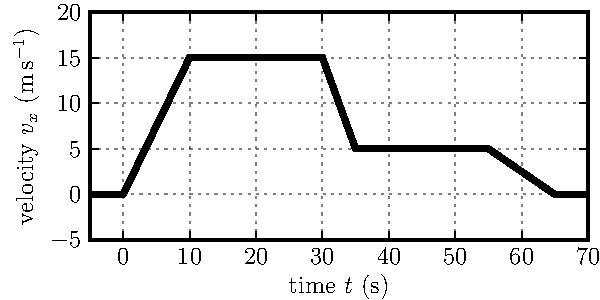
\includegraphics{../py/vx_vs_t.pdf}

\end{document}
